\section{Comparison with \cluestering{}}
\label{sec:cluestering}

\cluestering{} is a generalized, heterogeneous implementation of the CLUE
approach, with configurable coordinates and distance metrics. It retains the
density, nearest-higher and seed--follower structure introduced in
Section~\ref{sec:clue3d}, while allowing the neighbourhood geometry to be
changed. My work was to run and diagnose its application to displaced showers
in CMSSW, comparing several configurations with default \cluethreed{}.
The framework can use Cartesian positions directly or projective coordinates;
removing the origin assumption is therefore one possibility, rather than a
defining property of \cluestering{}.

\subsection{Cartesian distance metrics}

For Cartesian coordinates $(x,y,z)$, I explored three familiar distance
families. Writing $\Delta x=x_i-x_j$, and similarly for $y$ and $z$, their
unweighted forms are
\begin{align}
 D_2 &= \sqrt{\Delta x^2+\Delta y^2+\Delta z^2},\\
 D_1 &= |\Delta x|+|\Delta y|+|\Delta z|,\\
 D_\infty &= \max(|\Delta x|,|\Delta y|,|\Delta z|).
\end{align}
Euclidean distance $D_2$ measures straight-line separation, so a fixed distance
cut selects a sphere. Manhattan distance $D_1$ adds the separations along the
three axes and selects an octahedron. Chebyshev distance $D_\infty$ takes the
largest component and selects a cube: all three coordinate differences must
individually lie within the cut. These shapes give different neighbours even
when the numerical distance setting is identical.

Weights allow the longitudinal and transverse reaches to be adjusted. With
positive weights $w_k$ and coordinate differences $\Delta x_k$, the corresponding
forms are
\begin{align}
 D_{2,w} &= \sqrt{\sum_k w_k(\Delta x_k)^2},\\
 D_{1,w} &= \sum_k w_k|\Delta x_k|,\\
 D_{\infty,w} &= \max_k\bigl(w_k|\Delta x_k|\bigr).
\end{align}
The weighted examples shown below use $(w_x,w_y,w_z)=(1,1,2)$ for Euclidean
and Chebyshev distance; the Manhattan example is unweighted. Increasing the
longitudinal weight shortens the allowed reach in $z$. In these conventions,
a weight of two reduces the pure longitudinal reach by $\sqrt{2}$ for
Euclidean distance and by two for Chebyshev distance. All these Cartesian
metrics depend only on coordinate differences and make no projection towards
the interaction point.

\subsection{A projective metric under development}

I also tested a work-in-progress projective configuration, labelled
\emph{Gnomonic} in the plots. It maps LC positions to the direction coordinates
\begin{equation}
 \mathbf{g}=\left(\frac{x}{|z|},\frac{y}{|z|}\right),
\end{equation}
and uses the layer index $\ell$ as the longitudinal coordinate. Within one
endcap, the tested cylinder distance is
\begin{equation}
 D_{\mathrm{cyl}}(i,j)=\max\!\left(
 \frac{|\mathbf{g}_i-\mathbf{g}_j|}{\sigma_T},
 \frac{|\ell_i-\ell_j|}{L}\right).
 \label{eq:cluesteringcylinder}
\end{equation}
A cut $D_{\mathrm{cyl}}<d$ selects a transverse disc of radius $d\sigma_T$
and a longitudinal interval of half-height $dL$: a cylinder in the transformed
coordinate space. The transverse and longitudinal scales can thus be set
separately. Points on an ideal pointing shower have constant $\mathbf{g}$;
non-pointing showers drift across this plane, so some degradation with
displacement is still expected.

The tested implementation clusters only the electromagnetic section (EE).
It uses $\sigma_T=0.003$, $L=4$ layers, density radius $d_c=1$, seed distance
2.8 and outlier distance 3.6, with the distances expressed in the normalized
units of Eq.~\eqref{eq:cluesteringcylinder}, not centimetres. To account for PU $\eta$-uniform density, density
threshold also varies with direction:
\begin{equation}
 \rho_c(\mathbf{g})=\SI{0.8}{GeV}
       \left(\frac{0.42}{|\mathbf{g}|}\right)^2.
\end{equation}

\subsection{First comparisons without pileup}

These comparisons are exploratory tests of a few metrics and parameter
choices, not the result of tuning. For the Cartesian configurations,
I held the density radius at $d_c=5$~cm and the density threshold at
$\rho_c=6$~GeV, and concentrated on the nearest-higher distance $d_m$.
The preceding studies identified the distance reach as a particularly direct
control of fragmentation, making it the first parameter to vary before a
broader density-and-distance tuning. Unweighted and weighted Euclidean
metrics were tested at $d_m=3$ and 6~cm; Manhattan and weighted Chebyshev
are shown at 6~cm. Default parameters are used for \cluethreed{}, which is the baseline.

\begin{figure*}[!tp]
  \centering
  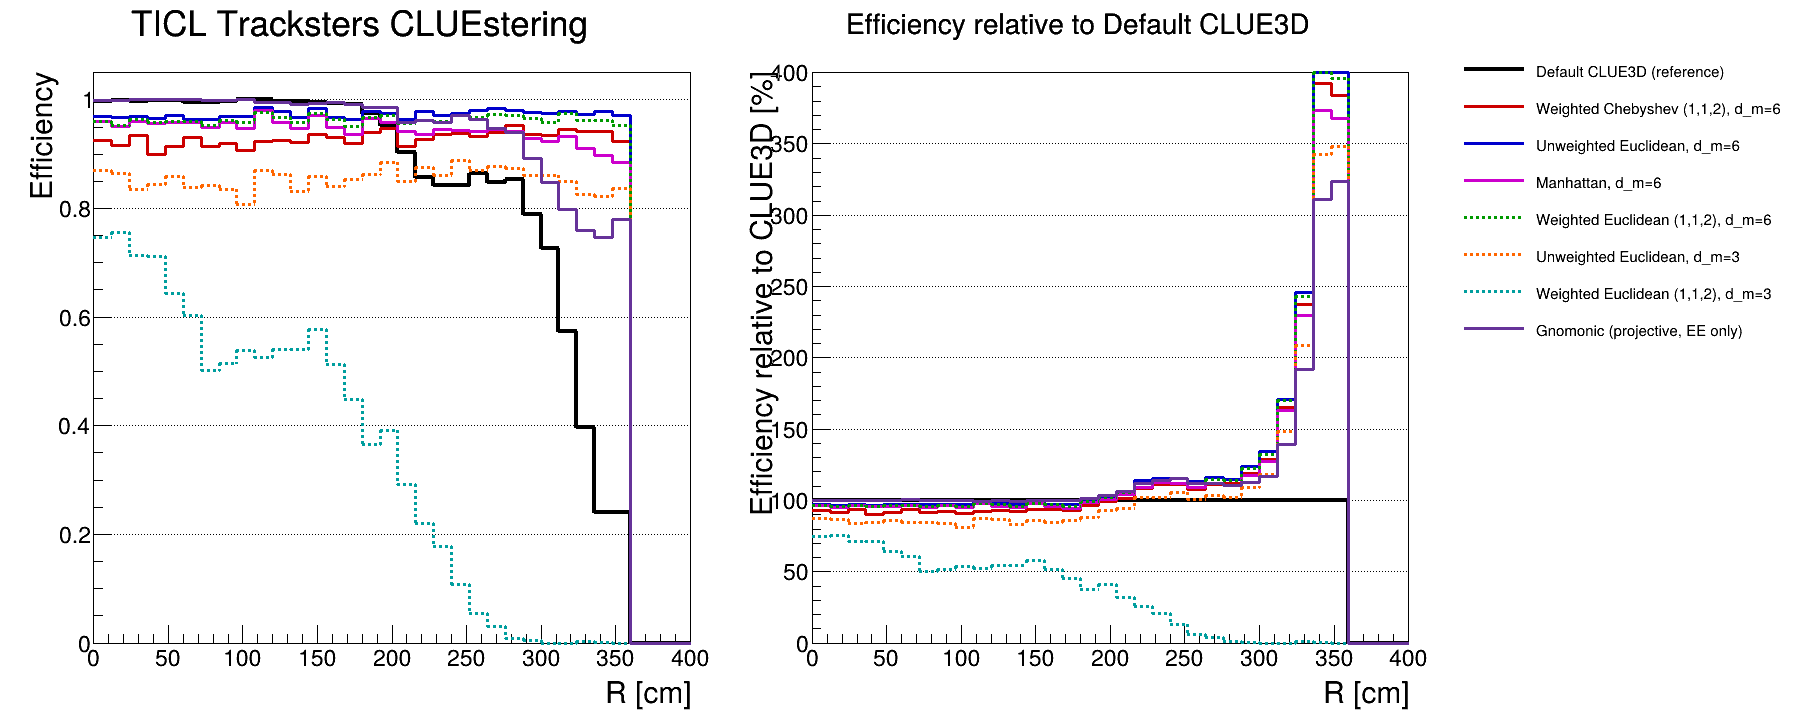
\includegraphics[width=\textwidth]{figures/cluestering_no_pu.png}
  \caption{Single-photon efficiency without pileup for the exploratory
  \cluestering{} configurations, including the EE-only gnomonic configuration,
  with default \cluethreed{} as the baseline. The right panel shows
  $100\,\epsilon/\epsilon_{\mathrm{CLUE3D}}$; $100\%$ denotes equal efficiency.
  The generated displacement scan ends at 350~cm.}
  \label{fig:cluesteringefficiencies}
\end{figure*}

The no-pileup comparison uses 20\,000 generated single-photon events with
energies of 10--250~GeV and $\R=0$--350~cm in Run4D121 geometry, subject to
the gun's surface-acceptance requirements. Figure~\ref{fig:cluesteringefficiencies}
shows that the 6~cm Cartesian configurations largely avoid the severe
large-displacement loss of \cluethreed{}. The two Euclidean variants retain
efficiencies in the mid-to-high $90\%$ range over most of the scan; Manhattan
and weighted Chebyshev also remain efficient, with somewhat lower curves.
These simple choices already show that the default \cluethreed{} behaviour
is not an unavoidable consequence of a displaced shower.

The gnomonic configuration performs well near the origin and degrades at
large displacement, as expected for projective coordinates. Its decline is
much less severe than that of \cluethreed{}, however, so this first test also
looks promising. Sharing an origin projection does not imply identical
performance: the cylinder neighbourhood, distance scales and density
prescription differ from those of \cluethreed{}.

The surprise is the smaller Euclidean distance setting. Unweighted Euclidean
at 3~cm is less efficient than at 6~cm, while the weighted 3~cm configuration
loses almost all efficiency by approximately 300~cm. Since it uses Cartesian
coordinates, this failure cannot be attributed to an origin projection.

\subsection{Understanding the weighted Euclidean 3 cm failure}

\begin{figure*}[!tp]
  \centering
  \begin{subfigure}{0.49\textwidth}
    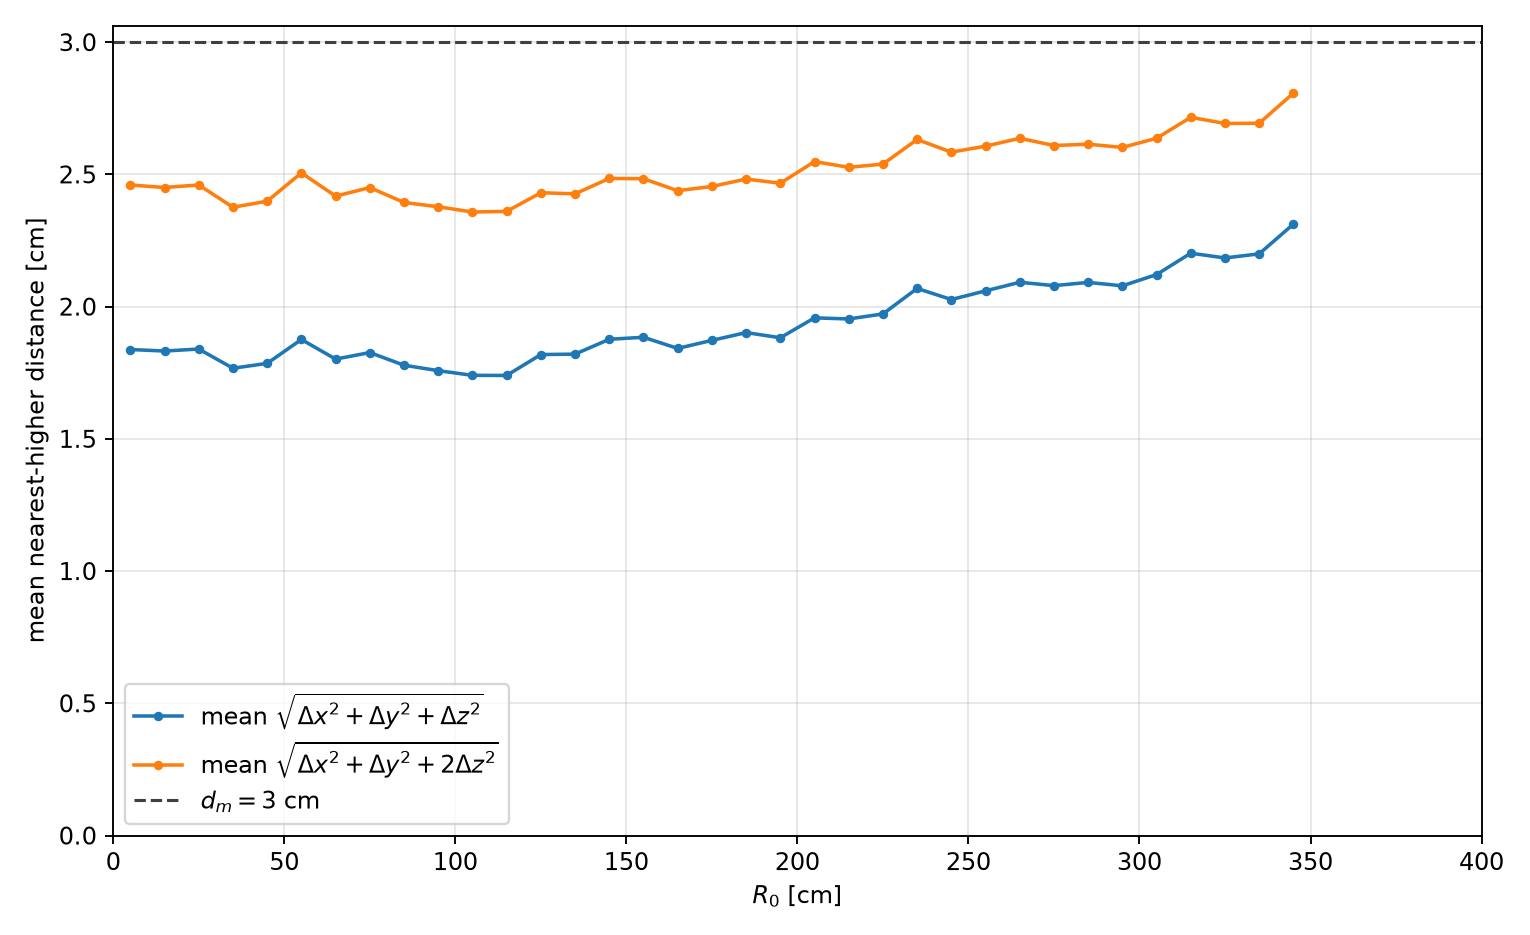
\includegraphics[width=\linewidth]{figures/cluestering_link_distances.png}
    \caption{Mean nearest-higher link distance, unweighted and weighted.}
  \end{subfigure}\hfill
  \begin{subfigure}{0.49\textwidth}
    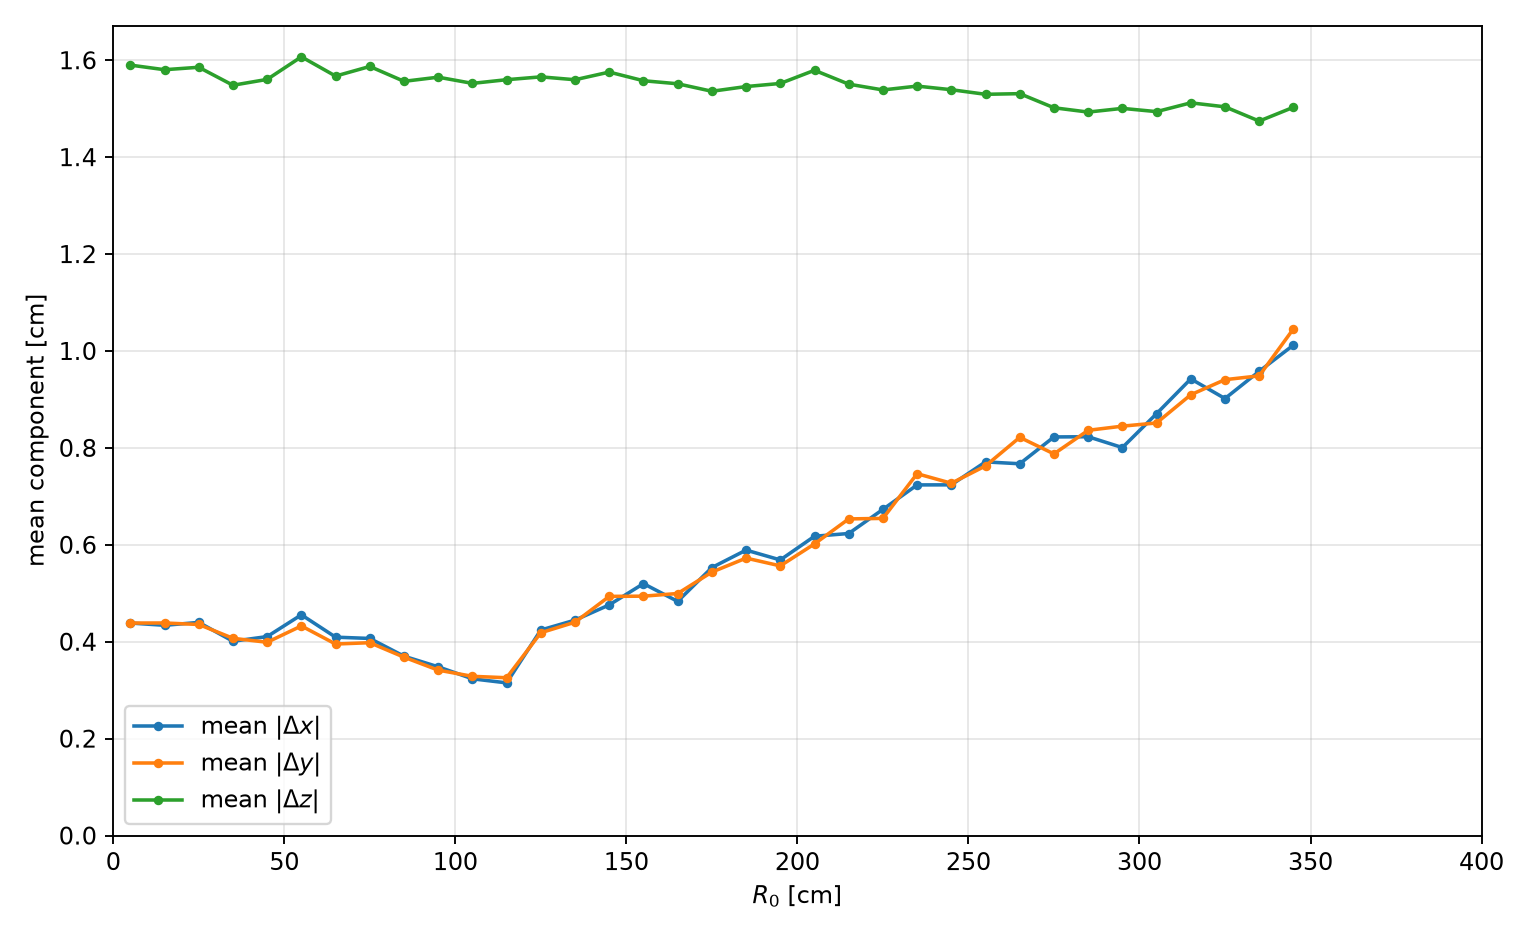
\includegraphics[width=\linewidth]{figures/cluestering_link_components.png}
    \caption{Mean absolute components of the nearest-higher link.}
  \end{subfigure}
  \par\medskip
  \begin{subfigure}{0.49\textwidth}
    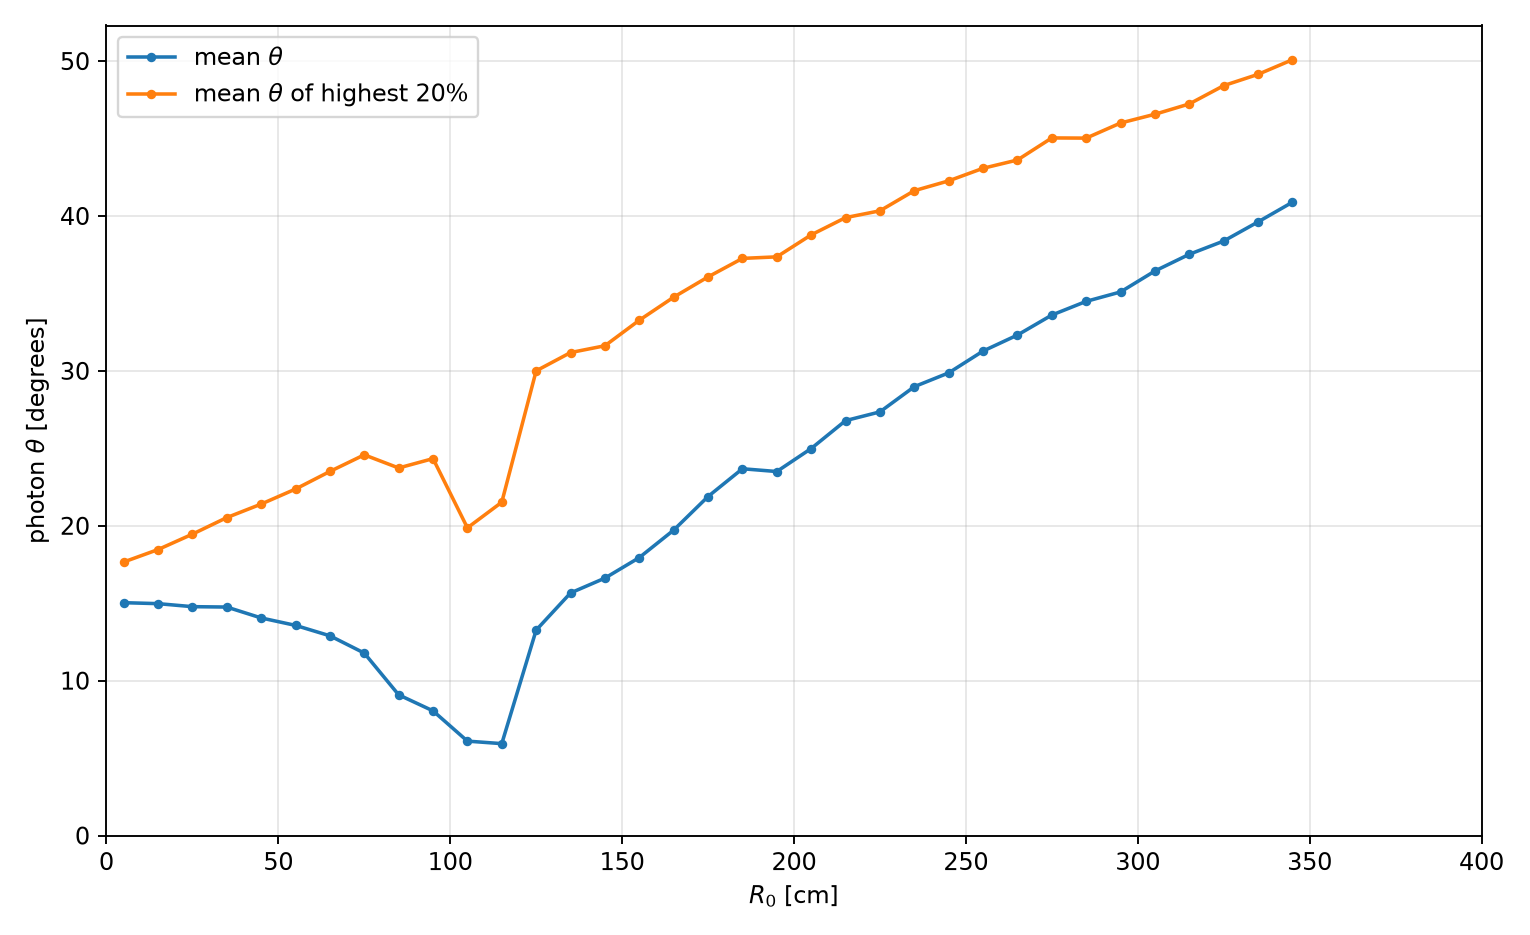
\includegraphics[width=\linewidth]{figures/cluestering_photon_theta.png}
    \caption{Mean photon angle $\theta$, and the mean of its most-inclined fifth.}
  \end{subfigure}\hfill
  \begin{subfigure}{0.49\textwidth}
    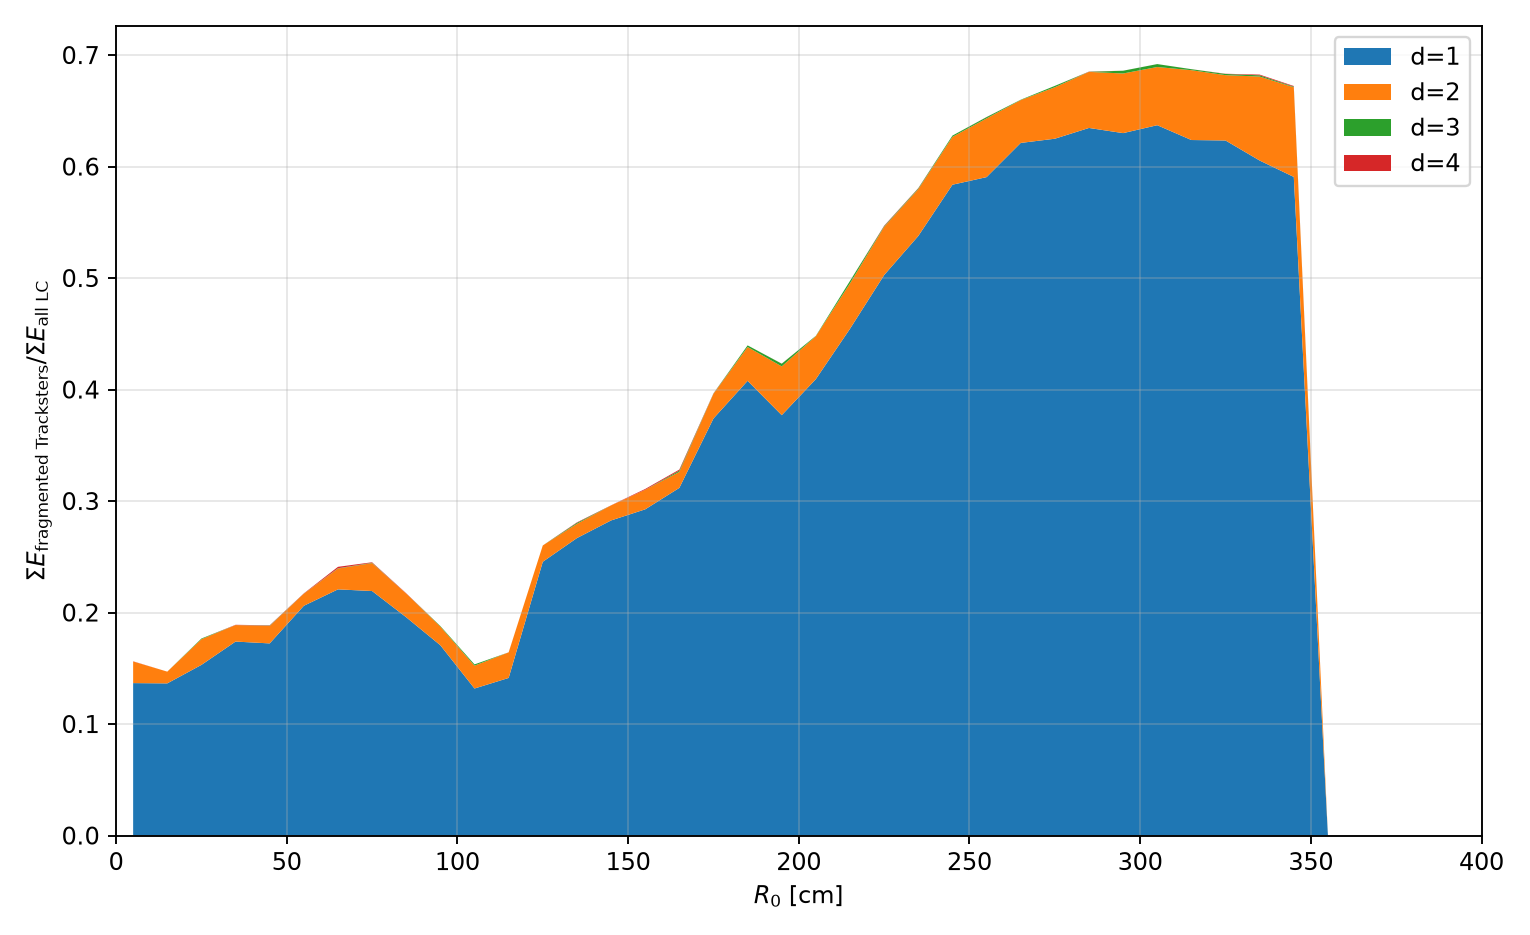
\includegraphics[width=\linewidth]{figures/cluestering_fragment_energy.png}
    \caption{Fraction of shower energy split into fragments, by the layer gap
    of the broken link.}
  \end{subfigure}
  \caption{Diagnostics for the weighted Euclidean metric at $d_m=3$~cm, versus
  truth displacement $R_0$. Panels (a) and (b) use only valid nearest-higher
  links. Panel (d) sums the full energy of the clusters rooted at seeds whose
  higher-density continuation lies beyond the 3~cm reach, normalized to the
  total LC energy; the label $d$ in its legend is the physical layer gap of the
  broken link.}
  \label{fig:cluesteringdiagnostic}
\end{figure*}

To understand why, I examined the nearest-higher links: their distance, their
separate coordinate components, and the shower energy that ends up in the
fragments they produce (Fig.~\ref{fig:cluesteringdiagnostic}). The links tell a
simple geometric story. An inclined shower advances along a tilted axis, so
consecutive layers are offset not only in $z$ but also transversely. For a
layer gap $\Delta z$, this transverse step is
\begin{equation}
 \Delta r_{xy}\simeq|\Delta z|\tan\theta,
 \label{eq:cluesteringangle}
\end{equation}
where $\theta$ is the photon polar angle. The HGCal layer spacing fixes the
longitudinal part of each link, while a larger inclination---which is what a
larger displacement produces---adds transverse distance. Panel~(b) shows
exactly this: at large $\R$ the transverse components grow while the
longitudinal one barely changes. Once the transverse step outgrows the 3~cm
reach, the link is cut and a single continuous shower is split---even though
nothing here projects towards the origin. The failure is therefore not really
inherent to displaced particles, but to particles with large $\theta$, which
displaced particles simply tend to have.

One thing looks paradoxical at first: the mean weighted link distance stays
below 3~cm across the whole scan (panel~a), yet the efficiency collapses. The
resolution is that clustering acts on individual links, and an average
comfortably under the threshold can still hide many links above it. The start
of the scan makes the point: below about 100~cm the mean photon angle and the
mean link distance both fall, yet the most inclined fifth of the photons moves
to larger $\theta$ (panel~c). It is this growing angular tail, not the average
shower, that runs into the distance limit.

The fragmentation diagnostic ties this link-level failure to the lost energy
(panel~d). The energy in clusters that hang off a seed whose higher-density
continuation lies beyond the reach rises to about two thirds of the total
shower energy at large displacement, dominated by continuations just one layer
away. A large part of each shower is therefore broken off into separate
objects. The lesson of the 3~cm test is that Cartesian coordinates remove the
artificial projective separation, but the distance reach and metric weights
must still be large enough to follow an inclined shower from one layer to the
next. This is a concrete target for future tuning.

\subsection{Performance in pileup}

The PU200 comparison uses a 10\,000-event sample for each tested
configuration. As in Section~\ref{sec:pileup}, I measured the generated signal
photon separately from the inclusive in-time truth population, and added two
complementary rates: signal-photon duplicates and reconstructed-object merges.
The signal measurement tests recovery of the displaced photon in a busy event;
the inclusive one tests the response to the many additional showers.

\begin{figure*}[!tp]
  \centering
  \begin{subfigure}{\textwidth}
    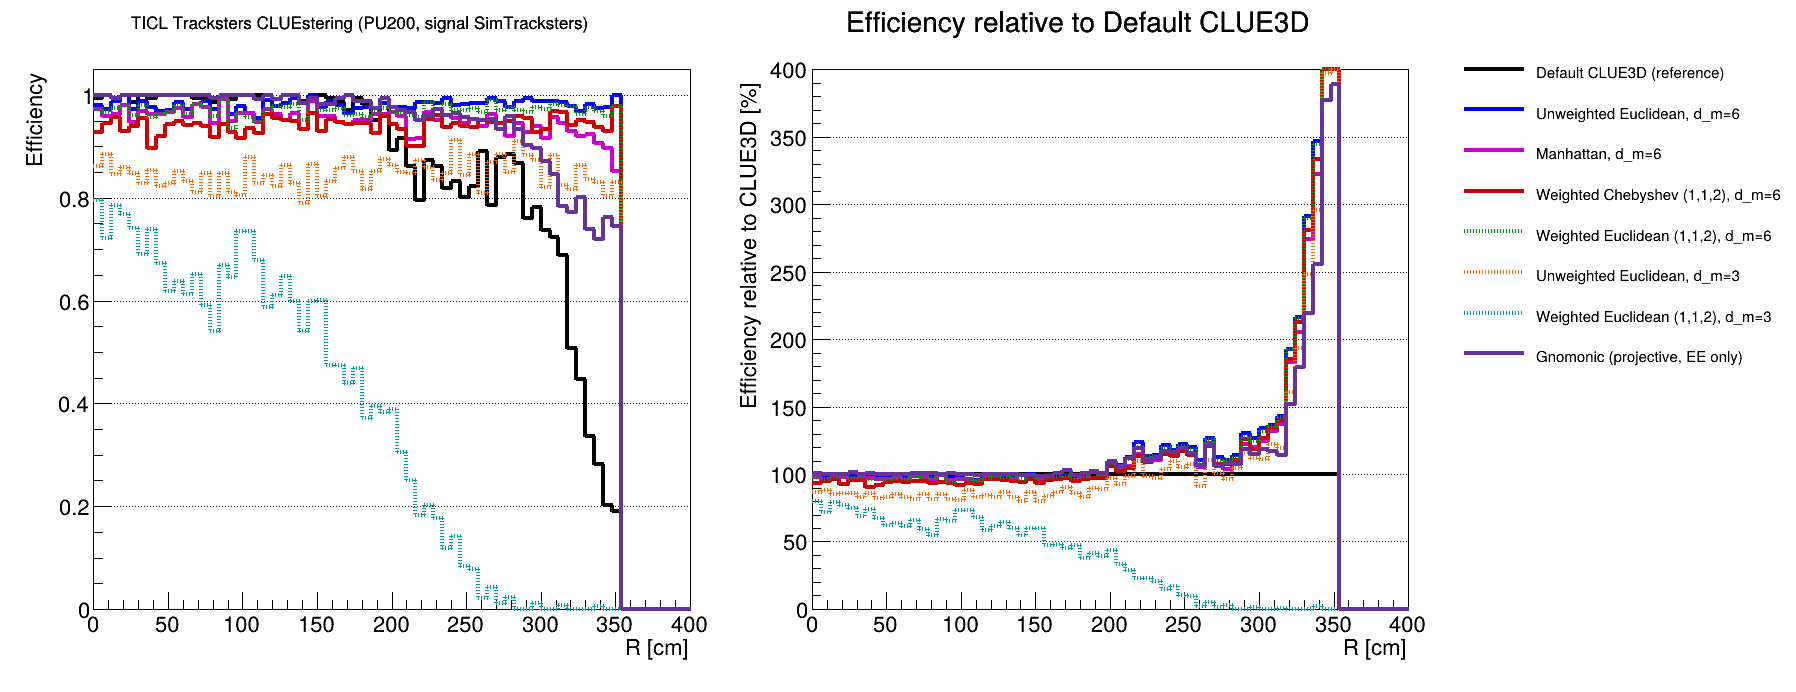
\includegraphics[width=\linewidth]{figures/cluestering_signal_pu.png}
    \caption{Efficiency for the generated signal photon in PU200.}
    \label{fig:cluesteringsignalpu}
  \end{subfigure}
  \par\medskip
  \begin{subfigure}{\textwidth}
    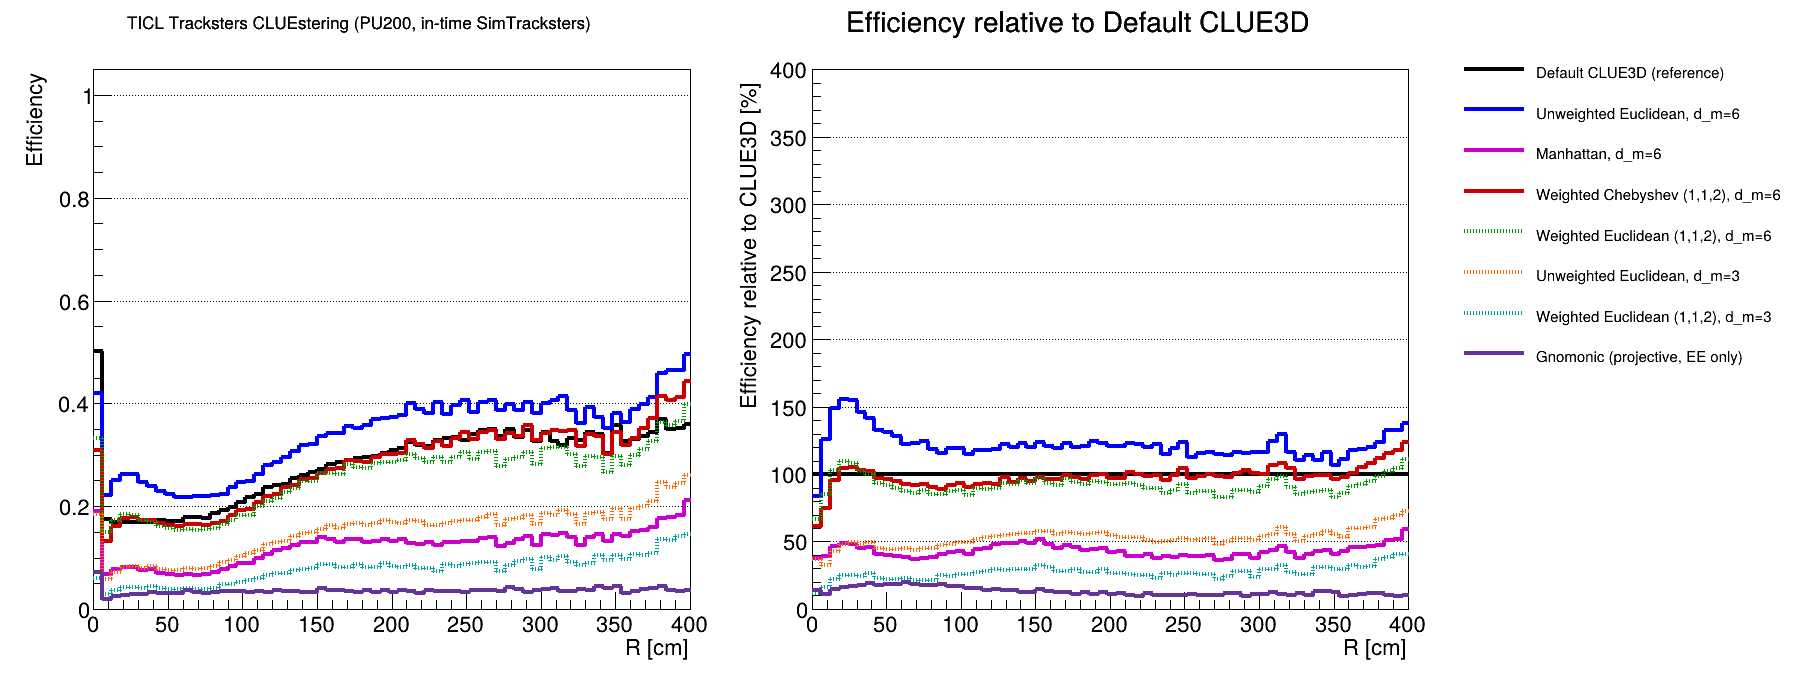
\includegraphics[width=\linewidth]{figures/cluestering_inclusive_pu.png}
    \caption{Efficiency for the inclusive in-time truth population.}
    \label{fig:cluesteringinclusive}
  \end{subfigure}
  \caption{PU200 efficiencies, with default \cluethreed{} as the baseline
  and the same relative-efficiency convention as
  Fig.~\ref{fig:cluesteringefficiencies}. The inclusive denominator includes
  showers in the hadronic sections, which the tested EE-only gnomonic
  configuration does not cluster.}
  \label{fig:cluesteringpuefficiencies}
\end{figure*}

For the signal photon, the no-pileup ordering survives
(Fig.~\ref{fig:cluesteringsignalpu}): the 6~cm Cartesian configurations stay
efficient across the scan, the gnomonic configuration again beats
\cluethreed{} at large displacement, and the weighted Euclidean 3~cm failure
is still present. Pileup does not remove the geometric limitations, nor does
it erase the gains of the more successful configurations.

The inclusive picture is different (Fig.~\ref{fig:cluesteringinclusive}). The
6~cm Cartesian metrics remain competitive---unweighted Euclidean improves on
\cluethreed{} over most of the range and weighted Chebyshev is broadly
comparable---while Manhattan and the 3~cm choices recover much less. The
gnomonic configuration is the striking outlier: even though its signal
efficiency is the \emph{higher} of the two, it collects only a small fraction
of the inclusive population, several times less than \cluethreed{} does.

This is unlikely to be the projective metric itself. We assume its direction-dependent
density threshold further suppresses much of the pileup, and it also hasn't been set up for hadronic subdetector which is relevant for PU. These are working
explanations rather than conclusions, confirming them requires further
checks.

\begin{figure*}[!tp]
  \centering
  \begin{subfigure}{0.49\textwidth}
    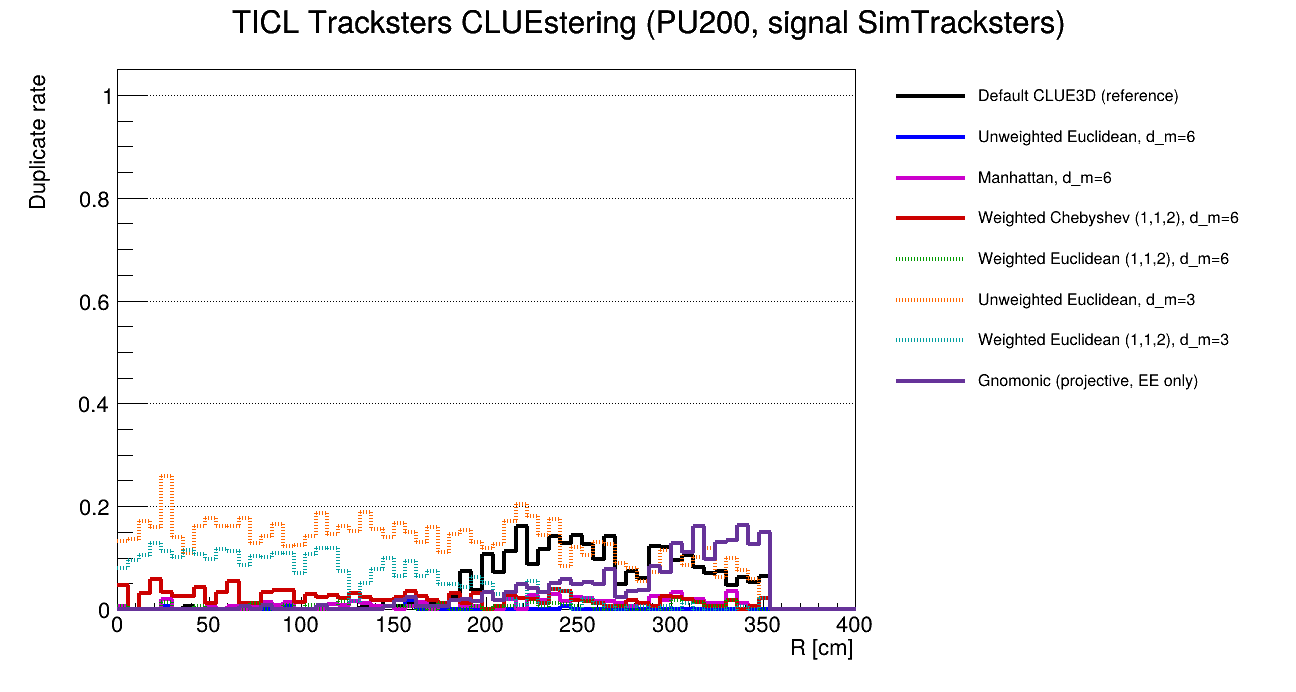
\includegraphics[width=\linewidth]{figures/cluestering_duplicates.png}
    \caption{Signal-photon duplicates versus truth displacement.}
  \end{subfigure}\hfill
  \begin{subfigure}{0.49\textwidth}
    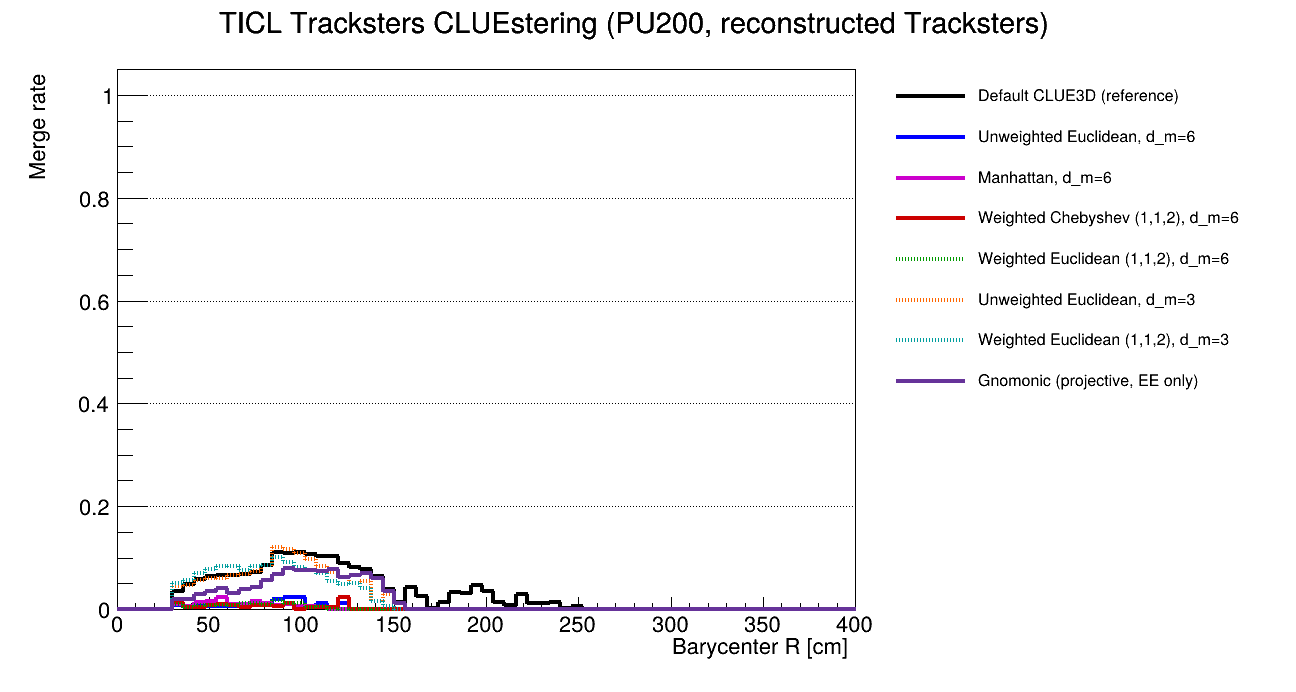
\includegraphics[width=\linewidth]{figures/cluestering_merges.png}
    \caption{Reconstructed-object merges versus barycentre radius.}
  \end{subfigure}
  \caption{Complementary PU200 rates. The duplicate denominator contains
  signal SimTracksters, while the merge denominator contains reconstructed
  Tracksters. The merge plot uses $\sqrt{x_c^2+y_c^2}$, the transverse radius
  of the Trackster barycentre, rather than its back-extrapolated displacement
  at $z=0$.}
  \label{fig:cluesteringrates}
\end{figure*}

The duplicate rates in Fig.~\ref{fig:cluesteringrates}(a) show how completely
the signal is collected into one object. The 6~cm Cartesian configurations
remain close to zero, whereas the 3~cm choices have appreciable duplicates
at small and intermediate displacement. Gnomonic duplicates rise at large
$\R$, consistent with its remaining projective fragmentation; its efficiency
gain over \cluethreed{} does not mean that every photon is recovered as one
Trackster.

The reconstructed-object merge curves in Fig.~\ref{fig:cluesteringrates}(b)
are small for the 6~cm Cartesian choices. Gnomonic and the 3~cm curves show
more merging, with gnomonic broadly comparable in size to \cluethreed{}.
These rates describe the surviving reconstructed objects, so their
interpretation must account for the very different object populations and
the efficiency loss. In particular, suppressing pileup objects can reduce
opportunities to count merges without establishing better shower separation.

\subsection{Two nearby photons and outlook}

\begin{figure*}[!tp]
  \centering
  \begin{subfigure}{0.49\textwidth}
    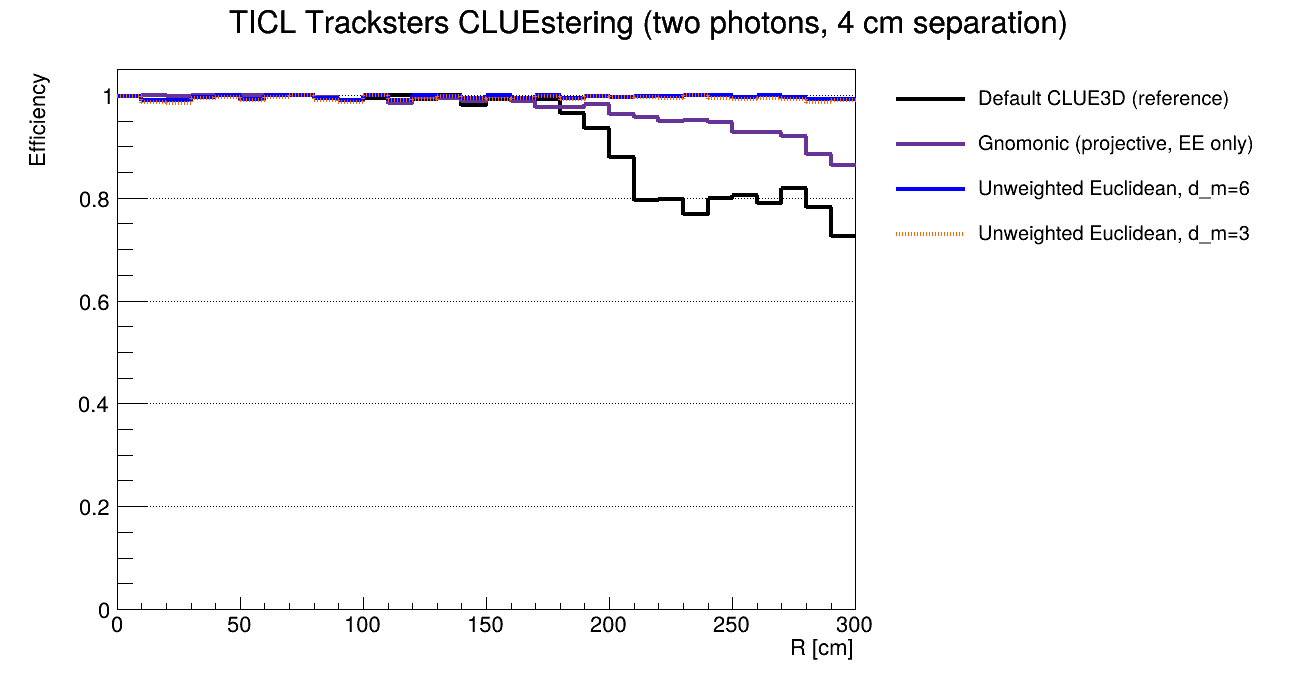
\includegraphics[width=\linewidth]{figures/cluestering_two_photon_efficiency.png}
    \caption{Photon reconstruction efficiency.}
  \end{subfigure}\hfill
  \begin{subfigure}{0.49\textwidth}
    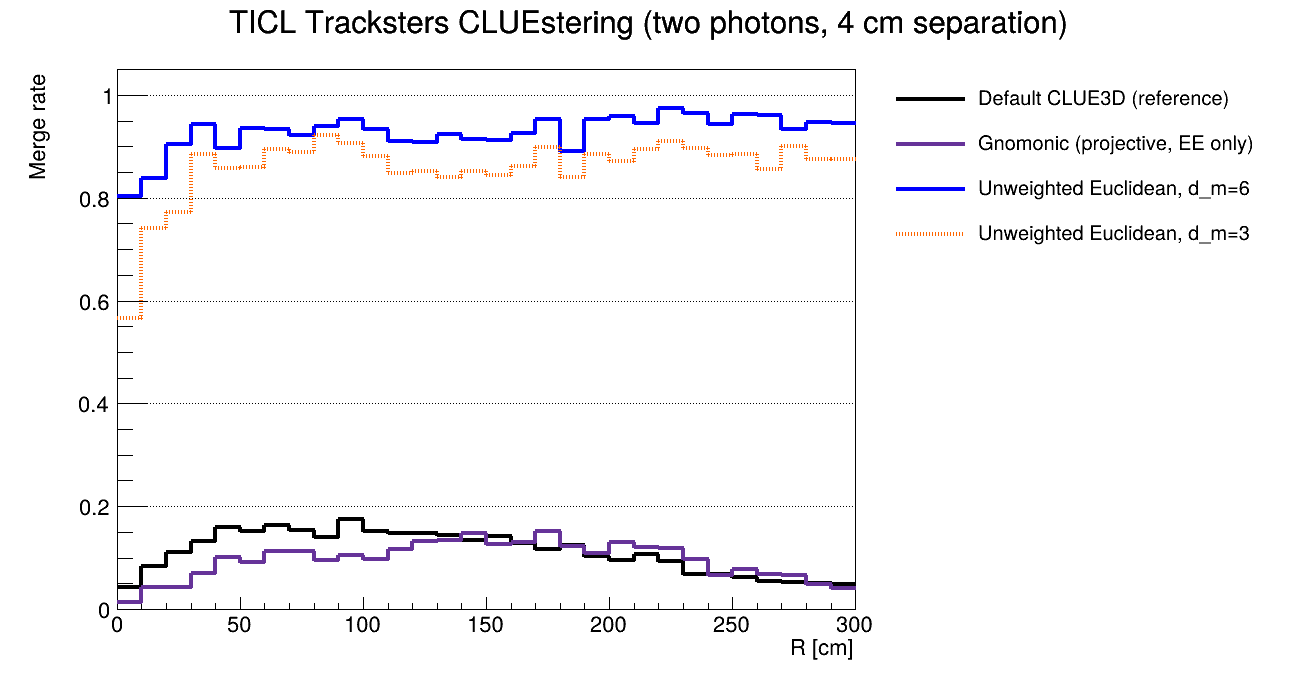
\includegraphics[width=\linewidth]{figures/cluestering_two_photon_merges.png}
    \caption{Reconstructed-object merge rate.}
  \end{subfigure}
  \caption{Two photons separated by 4~cm: photon efficiency and
  reconstructed-object merge rate for default \cluethreed{}, the gnomonic
  configuration, and unweighted Euclidean at $d_m=6$ and $3$~cm. Efficiency is
  binned in truth displacement and merge rate in reconstructed displacement,
  with 10~cm bins over 0--300~cm. The merge denominator contains nonempty
  Tracksters.}
  \label{fig:cluesteringtwophoton}
\end{figure*}

A dedicated two-photon comparison at 4~cm separation tests nearby showers
directly (Fig.~\ref{fig:cluesteringtwophoton}). Here efficiency cannot be read
on its own: two overlapping photons collected into a single object still count
as reconstructed, so a high efficiency can just as easily mean good recovery or
outright merging. It has to be read together with the merge rate. On that
basis the gnomonic configuration holds up well: at large displacement it keeps
higher efficiency than \cluethreed{} while its merge rate stays low and close
to \cluethreed{}'s. It recovers more of each photon without merging the two
together.

The Cartesian Euclidean metrics make the point in reverse. Unweighted Euclidean
at $d_m=6$~cm reaches near-perfect efficiency, but its merge rate is very high:
the wide reach simply clusters both showers into one object, which is exactly
what made it look so strong on single photons. More surprising is $d_m=3$~cm.
Its short reach fragmented a single shower earlier, yet with two photons its
efficiency climbs back to near unity while it merges almost as heavily as the
6~cm case. The likely explanation is that the neighbouring photon bridges the
gap: activity from the second shower fills the spacing that a 3~cm reach could
not span alone, reconnecting the fragments into one merged object. This would
need a dedicated study to confirm.

As shown in Section~\ref{sec:merging}, fragmentation can also hide mixing
inside an object-based merge rate, so extending the cross-shower LC-link
diagnostic to these configurations would test separation more directly. Taken
together, the results show that \cluestering{} offers several useful choices:
the gnomonic configuration improves on \cluethreed{} in both single- and
two-photon tests, while the Cartesian metrics buy their high efficiency partly
by merging and must be tuned against that. Its strong suppression of the pileup remains a limitation of the present setup. The next
step is to extend the input coverage and tune coordinates, metric weights,
distance reaches and density settings together, using signal and PU efficiency, duplicate, merge and fake rate to guide the choice.
